\documentclass[border=8pt]{standalone}
\usepackage{pgfplots}
\pgfplotsset{compat=1.18}
\begin{document}
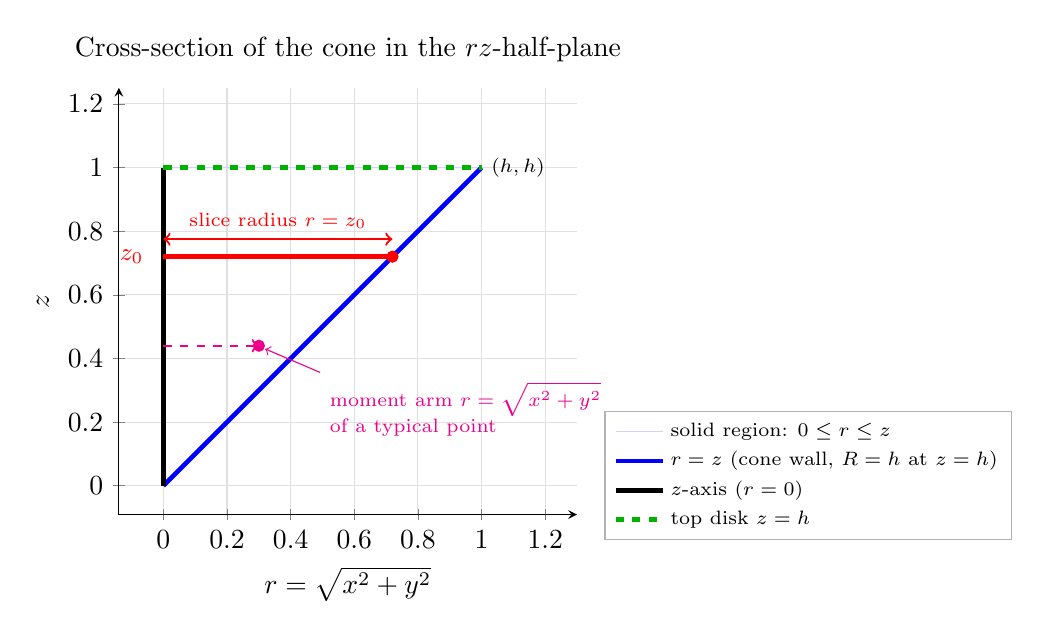
\begin{tikzpicture}
\begin{axis}[
  width=7.4cm, height=7.0cm, axis lines=left,
  xlabel={$r=\sqrt{x^2+y^2}$}, ylabel={$z$},
  xmin=-0.14, xmax=1.30, ymin=-0.06, ymax=1.22,
  xtick={0,0.2,...,1.2}, ytick={0,0.2,...,1.2},
  axis equal, grid=both, grid style={black!12},
  legend style={at={(1.06,-0.06)},anchor=south west,font=\scriptsize,draw=black!30,fill=white},
  legend cell align=left,
  title={Cross-section of the cone in the $rz$-half-plane},
  clip=false]
  \addplot[blue!18, fill opacity=0.85] coordinates {(0,0) (1,1) (0,1)} \closedcycle;
  \addlegendentry{solid region: $0\le r\le z$}
  \addplot[blue, ultra thick, domain=0:1, samples=2] ({x},{x});
  \addlegendentry{$r=z$ (cone wall, $R=h$ at $z=h$)}
  \addplot[black, ultra thick] coordinates {(0,0) (0,1)};
  \addlegendentry{$z$-axis ($r=0$)}
  \addplot[green!70!black, ultra thick, dashed] coordinates {(0,1) (1,1)};
  \addlegendentry{top disk $z=h$}
  % representative horizontal slice at z0
  \addplot[red, ultra thick] coordinates {(0,0.72) (0.72,0.72)};
  \addplot[red, only marks, mark=*] coordinates {(0.72,0.72)};
  \draw[<->,red,thick] (0,0.775) -- (0.72,0.775) node[midway,above,red,font=\scriptsize]{slice radius $r=z_0$};
  \node[red,font=\small] at (axis cs:-0.10,0.72) {$z_0$};
  \node[font=\scriptsize,right] at (axis cs:1,1) {$(h,h)$};
  % typical interior point and its moment arm about the z-axis
  \draw[magenta, thick, dashed,->] (0,0.44) -- (0.30,0.44);
  \addplot[magenta, only marks, mark=*] coordinates {(0.30,0.44)};
  \node[magenta,font=\scriptsize,align=left] (lab) at (axis cs:0.95,0.24)
     {moment arm $r=\sqrt{x^2+y^2}$\\ of a typical point};
  \draw[magenta,thin,->] (lab.north west) -- (0.32,0.43);
\end{axis}
\end{tikzpicture}
\end{document}
